\documentclass[a4paper,11pt]{article}

\usepackage[T1]{fontenc} 
\usepackage[utf8]{inputenc}

\usepackage{listings} \lstset{language=c, showstringspaces=false, xleftmargin=-0pt, frame=l}

\usepackage{graphicx}
\usepackage{lmodern}

\usepackage{calc}
\usepackage{bytefield}

\usepackage{listings} \lstset{
  language=c, 
  basicstyle=\ttfamily\small,
  showstringspaces=false
}


\usepackage{tikz}
\usetikzlibrary{arrows}
\usetikzlibrary{topaths}
\usetikzlibrary{calc}
\usetikzlibrary{positioning}


\begin{document}

\begin{center} \vspace{20pt} \textbf{\large The magical mystery tour}\\
\vspace{10pt} \textbf{Johan Montelius}\\ \vspace{10pt} \textbf{HT2018}
\end{center}


\section{Introduction}

In this assignment you're going to implement a smart version of {\em
  malloc()}. The trick we will use is to store additional information
about block sizes in order for us to easily find the neighboring
blocks when performing the {\em free()} operation. You should have a
good understanding of what malloc and free should do, and preferably
you should have tried to implement them.

The implementation will follow the ideas used by Doug Lea in his {\em
  dlmalloc}. This was for long time the default memory allocator in
Linux but has since many years been replaced by the updated version
called {\em ptmalloc3}. The difference between our simple allocator
and the more advanced schemes is mainly in how to deal with multiple
threads. The simple version that you will implement will give you the
basic idea of how things are handled.

\section{The structure}

The main idea is that we should be able to locate the blocks
immediately before and after a given block. The block that is located
after a given block can be found if know the size of the given
block. This should be simple since we some how need to keep track of
the size of a block anyway. It's a bit more tricky to find the block
that is located immediately before the block since it requires that we
know the size of that block. We solve this by also keeping track of
the size of this block but we have to remember to update it.


All free blocks will be kept in a double linked list since we want to
be able to remove a block without searching for its position if we
want to remove a block. We will in the first incarnation of the
implementation work with only one list and pick the first that we find
but this is something that you could improve later.

\subsection{a block}

A block starts with a {\em head} structure. This header holds:

\begin{itemize}
\item {\em footer} : the size of the block immediately before the block
\item {\em size} : the size of the block
\item {\em merge} : if we can merge with the block before the block or not (M/X)
\item {\em free} : if the block is free or taken (F/T)
\end{itemize}

The {\em footer} has a strange name for something that is first in a
block but if you view it as part of the block before it makes
sence. In the original description of this algorithm it is part of
that block and we keep the terminology.

The {\em free flag} tells us if the block is {\em Free} to use or {\em
  Taken} by a user process. The merge flag will tell us if we could
{\em Merge} the block with the block immediately before the block. If
the block immediately before the block is taken, then we should not
({\em X}) try to merge the blocks.

A free block will have two additional fields, the two pointers
needed to link to free blocks in the freelist.

\begin{itemize}
\item {\em next} : a pointer to the next block
\item {\em prev} : a pointer to the previous block
\end{itemize}
  
This all sounds easy, and so far it is, but we will complicate things -
don't worry. We start by looking at how large the different fields
need to be. We keep things aligned on {\em word} boundaries, and a word
will in our implementation be eight bytes. Let's store the footer in
one word, the size and flags in one word and the two pointers in one
word each. The outline of a free block of size 6 is shown in Figure~\ref{fig:head}. The first field holds the size of the block before but
since the merge flag is cleared (X) we don't really care what size it
has.

\begin{figure}[t]
\begin{center}
  \begin{tikzpicture}
    \coordinate (free) at (2,3);

    \draw[] (free) ++(0,-1)-- ++(0,3.9) -- ++(2,0) -- ++(0,-3.9);
    
    \draw[dashed] (free)++(0.1,2.2) rectangle +(1.8,0.6) node[midway] { ... };
    \draw[dashed] (free)++(0.1,1.5) rectangle +(1.8,0.6) node[midway] {6 / X / F};
    \draw[dashed] (free)++(0.1,0.8) rectangle +(1.8,0.6) node[midway] {next};
    \draw[->] (free)++(1.6,1.1) -- ++(1.6,0);
    \draw[dashed] (free)++(0.1,0.1) rectangle +(1.8,0.6) node[midway] {prev};
    \draw[->] (free)++(0.4,0.4) -- ++(-1.6,0);

    \coordinate (taken) at (8,3);

    \draw[] (taken) ++(0,-1)-- ++(0,3.9) -- ++(2,0) -- ++(0,-3.9);
    
    \draw[dashed] (taken)++(0.1,2.2) rectangle +(1.8,0.6) node[midway] { ... };
    \draw[dashed] (taken)++(0.1,1.5) rectangle +(1.8,0.6) node[midway] {6 / X / T};
    \node[] at ($(taken)+(1,1)$) {data};
    \draw[dashed] (taken) ++(0.1,-1)-- ++(0,2.4) -- ++(1.8,0) -- ++(0,-2.4); 

    \coordinate (user) at (12,6);
    \node[anchor=south] at (user) {user};
    \draw[->] (user) to[out=270, in=0] ($(taken) +(2.2,1.1)$);

   \end{tikzpicture}
\end{center}
   \caption{Outline of block header fields}
   \label{fig:head} 
 \end{figure}

When we hand out a block to a user we only need to preserve the size
and flags of the block so the words for the pointers could be used for
user data. We will do the regular magic trick and return a pointer to
this field and thereby hide and protect the first part of the
header.

\subsection{the trick}

The smallest possible block is four words large since we need at least
this much space to hold the required fields. When we hand this block
out to a user only two words can be used which gives us a large
overhead. This is when we realize something and do a smart trick. The
footer field of the block after the current block is never needed when
the current block has been allocated to the user. The footer field is
only used when a block should merge with another block and no one will
ever try to merge with a taken block. We can thus use the footer field
of the following block for user data. The smallest block will thus
hold three words of user data.

Let's take a look at a free block that should be able to hold five
words; it would look like the left block block in
Figure~\ref{fig:block}. If we allocate this block we change the
status, use the next and previous links and also the footer of the
block after as shown to the right in Figure~\ref{fig:block}. Also note
that we clear the merge flag of the following block.

\begin{figure}[t]
\begin{center}
  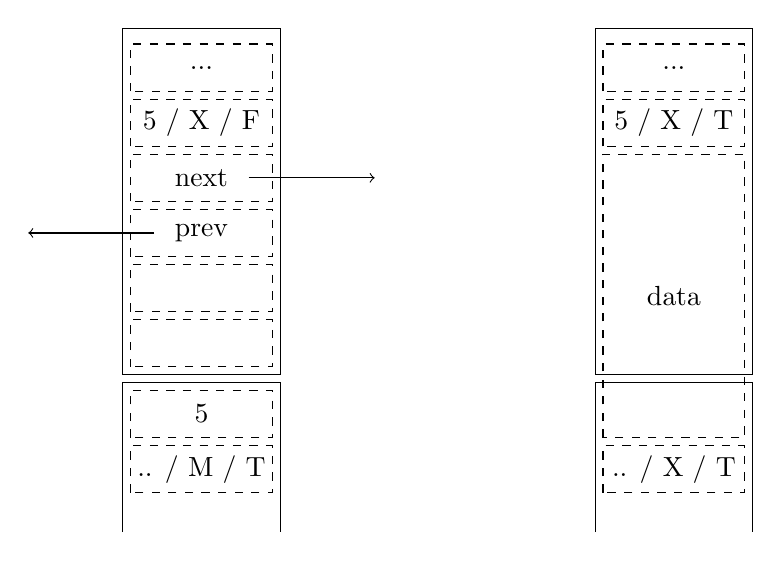
\begin{tikzpicture}
    \coordinate (taken) at (8,3);
    \coordinate (free) at (2,3);     

    
    \draw[] (free) rectangle +(2,4.4);
    \draw[dashed] (free)++(0.1,3.6) rectangle +(1.8,0.6) node[midway] { ... };
    \draw[dashed] (free)++(0.1,2.9) rectangle +(1.8,0.6) node[midway] {5 / X / F};
    \draw[dashed] (free)++(0.1,2.2) rectangle +(1.8,0.6) node[midway] {next};
    \draw[->] (free)++(1.6,2.5) -- ++(1.6,0);
    \draw[dashed] (free)++(0.1,1.5) rectangle +(1.8,0.6) node[midway] {prev};
    \draw[->] (free)++(0.4,1.8) -- ++(-1.6,0);
    \draw[dashed] (free)++(0.1,0.8) rectangle +(1.8,0.6);
    \draw[dashed] (free)++(0.1,0.1) rectangle +(1.8,0.6);
    
    \draw[] (free)++(0,-2) -- ++(0,1.9) -- ++(2,0) -- ++(0,-1.9);    
    \draw[dashed] (free)++(0.1,-0.8) rectangle +(1.8,0.6) node[midway] { 5 };
    \draw[dashed] (free)++(0.1,-1.5) rectangle +(1.8,0.6) node[midway] {.. / M / T};    

    \draw[] (taken) rectangle +(2,4.4);
    \draw[dashed] (taken)++(0.1,3.6) rectangle +(1.8,0.6) node[midway] { ... };
    \draw[dashed] (taken)++(0.1,2.9) rectangle +(1.8,0.6) node[midway] {5 / X / T};
    \draw[dashed] (taken)++(0.1,-0.8) rectangle +(1.8,3.6) node[midway] {data};

    \draw[] (taken)++(0,-2) -- ++(0,1.9) -- ++(2,0) -- ++(0,-1.9);
    \draw[dashed] (taken)++(0.1,-1.5) rectangle +(1.8,0.6) node[midway] {.. / X / T};
   \end{tikzpicture}
\end{center}
   \caption{A block of 5 words: free and taken}
   \label{fig:block} 
 \end{figure}

 
 \subsection{simple allocate and free}

 When a block is allocated we first find a suitable block that is
 large enough to serve the request of the user. In the simple case we
 find a block that is the right size and can then un-link it from the
 double linked list. We also need to update the status information of
 the block that comes after the block that we select. This block can
 be found since we know the size of the selected block. In the example
 with our five word block we would find the header of the following
 block at an address six words away.

 When we free a block we must reset this flag so also here would we
 have to find the following block. If these were the only operations
 it would be fairy pointless to maintain this information but we shall
 soon see how this extra status flag is used. 

 \subsection{merge blocks}

 
 If we free a block we should first take a look at the merge flag that
 tells us if the block before the current block is mergeable.  This
 can be done simply by incrementing the size of the block before the
 current block and set the footer correctly. The question is how we
 find the header of the block before us but this is where the copy of
 the size information helps us. If the block is mergable we should be
 able to trust the size information found in the footer.
 
\begin{figure}
\begin{center}
  \begin{tikzpicture}
    \coordinate (taken) at (2,3);
    \coordinate (before) at (2,7.1);
    \coordinate (user) at (0,7);
    
    \coordinate (free) at (8,3);     


    \draw[] (before) rectangle +(2,4.7) node[midway] {};
    \draw[dashed] (before)++(0.1,4.0) rectangle +(1.8,0.6) node[midway] {...};
    \draw[dashed] (before)++(0.1,3.3) rectangle +(1.8,0.6) node[midway] {6 / X / F};
    \draw[dashed] (before)++(0.1,2.6) rectangle +(1.8,0.6) node[midway] {next};
    \draw[->] (before)++(1.6,2.9) -- ++(1.6,0);
    \draw[dashed] (before)++(0.1,1.9) rectangle +(1.8,0.6) node[midway] {prev};
    \draw[->] (before)++(0.4,2.2) -- ++(-1.6,0);

    \draw[] (taken) rectangle +(2,4);
    \draw[dashed] (taken)++(0.1,3.3) rectangle +(1.8,0.6) node[midway] {6};    
    \draw[dashed] (taken)++(0.1,2.6) rectangle +(1.8,0.6) node[midway] {5 / M / T};
    \draw[dashed] (taken)++(0.1,-0.8) rectangle +(1.8,3.3) node[midway] {data};
 
    \draw[] (taken)++(0,-2) -- ++(0,1.9) -- ++(2,0) -- ++(0,-1.9);

    \node[anchor=south] at (user) {free};
    \draw[->] (user) to[out=270, in=180] ($(taken) +(-0.2,2.2)$);    
    
    \draw[] (free) rectangle +(2,8.8);
    \draw[dashed] (free)++(0.1,8.1) rectangle +(1.8,0.6) node[midway] {...};
    \draw[dashed] (free)++(0.1,7.4) rectangle +(1.8,0.6) node[midway] {12/ X / F};
    \draw[dashed] (free)++(0.1,6.7) rectangle +(1.8,0.6) node[midway] {next};
    \draw[->] (free)++(1.6,7.0) -- ++(1.6,0);
    \draw[dashed] (free)++(0.1,6.0) rectangle +(1.8,0.6) node[midway] {prev};
    \draw[->] (free)++(0.4,6.3) -- ++(-1.6,0);

    \draw[] (free)++(0,-2) -- ++(0,1.9) -- ++(2,0) -- ++(0,-1.9);    
    \draw[dashed] (free)++(0.1,-0.8) rectangle +(1.8,0.6) node[midway] {12};
   
    
   \end{tikzpicture}
\end{center}
   \caption{Merge a block with block before}
   \label{fig:mergebefore} 
 \end{figure}

 In Figure~\ref{fig:mergebefore} we see how a block of size five is
 merged with a free block of size six. The resulting block has a size
 of 12 since we gain one word that was used for the header. Not that
 the block before could not have a free block before it. If this was
 the case the two blocks should have been merged already.

 Regardless if we have merged with the block before the current block
 or not, we could still merge with the block after the current
 block. Since we know the size of the current block we should be able
 to find the header of the block after it and can then examine the
 status flag.
 
 If this block is free we can merge the two blocks. In order to do
 this we unlink the block from its position and instead insert the
 updated current block at this position as shown in Figure ~\ref{fig:mergeafter}.

 If the block is not free we will not be able to do a merge operation
 but we must change the state of the {\em merge} flag of the
 block. This is shown a in Figure~\ref{fig:nomerge}.
 
 \begin{figure}
\begin{center}
  \begin{tikzpicture}
    \coordinate (after) at (2,3);
    \coordinate (taken) at (2,7.1);

    \coordinate (user) at (0,7);
    
    \coordinate (free) at (8,3);     


    \draw[] (taken) rectangle +(2,4.7) node[midway] {};
    \draw[dashed] (taken)++(0.1,4.0) rectangle +(1.8,0.6) node[midway] {...};
    \draw[dashed] (taken)++(0.1,3.3) rectangle +(1.8,0.6) node[midway] {6/../T};
    \draw[dashed] (taken)++(0.1,-0.8) rectangle +(1.8,4.0) node[midway] {data};

    \node[anchor=north] at (user) {free};
    \draw[->] (user) to[out=90, in=180] ($(taken) +(-0.2,3.0)$);
    
    \draw[] (after) rectangle +(2,4);
    \draw[dashed] (after)++(0.1,2.6) rectangle +(1.8,0.6) node[midway] {5/X/F};
    \draw[dashed] (after)++(0.1,1.9) rectangle +(1.8,0.6) node[midway] {next};
    \draw[->] (after)++(1.6,2.2) -- ++(1.6,0);
    \draw[dashed] (after)++(0.1,1.2) rectangle +(1.8,0.6) node[midway] {prev};
    \draw[->] (after)++(0.4,1.5) -- ++(-1.6,0);

    \draw[] (after)++(0,-2) -- ++(0,1.9) -- ++(2,0) -- ++(0,-1.9);
    \draw[dashed] (after)++(0.1,-0.8) rectangle +(1.8,0.6) node[midway] {5};
    
    \draw[] (free) rectangle +(2,8.8);
    \draw[dashed] (free)++(0.1,8.1) rectangle +(1.8,0.6) node[midway] {...};
    \draw[dashed] (free)++(0.1,7.4) rectangle +(1.8,0.6) node[midway] {12/../F};
    \draw[dashed] (free)++(0.1,6.7) rectangle +(1.8,0.6) node[midway] {next};
    \draw[->] (free)++(1.6,7.0) -- ++(1.6,0);
    \draw[dashed] (free)++(0.1,6.0) rectangle +(1.8,0.6) node[midway] {prev};
    \draw[->] (free)++(0.4,6.3) -- ++(-1.6,0);

    \draw[] (free)++(0,-2) -- ++(0,1.9) -- ++(2,0) -- ++(0,-1.9);    
    \draw[dashed] (free)++(0.1,-0.8) rectangle +(1.8,0.6) node[midway] {12};
   
    
   \end{tikzpicture}
\end{center}
   \caption{Merge a block with block after}
   \label{fig:mergeafter} 
 \end{figure}


\begin{figure}
\begin{center}
  \begin{tikzpicture}

    \coordinate (taken) at (2,7.1);
    
    \coordinate (free) at (8,7.1);     

    \draw[] (taken) rectangle +(2,4.7) node[midway] {};
    \draw[dashed] (taken)++(0.1,4.0) rectangle +(1.8,0.6) node[midway] {...};
    \draw[dashed] (taken)++(0.1,3.3) rectangle +(1.8,0.6) node[midway] {6/X/T};
    \draw[dashed] (taken)++(0.1,-0.8) rectangle +(1.8,4.0) node[midway] {data};

    \draw[] (taken)++(0,-2) -- ++(0,1.9) -- ++(2,0) -- ++(0,-1.9);
    \draw[dashed] (taken)++(0.1,-1.5) rectangle +(1.8,0.6) node[midway] {../X/T};

    
    \draw[] (free) rectangle +(2,4.7);
    \draw[dashed] (free)++(0.1,4.0) rectangle +(1.8,0.6) node[midway] {...};
    \draw[dashed] (free)++(0.1,3.3) rectangle +(1.8,0.6) node[midway] {6/X/F};
    \draw[dashed] (free)++(0.1,2.6) rectangle +(1.8,0.6) node[midway] {next};
    \draw[->] (free)++(1.6,2.9) -- ++(1.6,0);
    \draw[dashed] (free)++(0.1,1.9) rectangle +(1.8,0.6) node[midway] {prev};
    \draw[->] (free)++(0.4,2.2) -- ++(-1.6,0);

    \draw[] (free)++(0,-2) -- ++(0,1.9) -- ++(2,0) -- ++(0,-1.9);    
    \draw[dashed] (free)++(0.1,-0.8) rectangle +(1.8,0.6) node[midway] {6};
    \draw[dashed] (free)++(0.1,-1.5) rectangle +(1.8,0.6) node[midway] {../M/T};
    
   \end{tikzpicture}
\end{center}
   \caption{No merge possible}
   \label{fig:nomerge} 
 \end{figure}

 
 These two operations could of course be combined so from three blocks
 we end up with one block. The pseudo code for the merge operation could look as follows:

 \begin{lstlisting}
merge( current ) {
  if( merge with before ) {
    if ( after is free ) {
      remove after from freelist
      update size of before
    } else {
      update size of before
      set merge flag of after
    }
    update footer
  } else {
    if ( after is free ) {
      update size of current
      let current take position of after
    } else {
      set merge flag of after
      place current in freelist
    }
    set current status to free
    update footer
  }
}
\end{lstlisting}


\subsection{splitting a block}

When we allocate a new block we first search through the list of free
block until we find one that is large enough to suit our needs. It
could be that this block is larger than what we need and we should
then split it and leave the part that we do not need. It is of course
pointless to leave something that is too small to handle but as long
as it is large enough to form a block we will do the split. In the
structure that we have outlined the smallest block would hold three user
data fields (one that is the footer of the next header). 

If we find a block that needs to be split we perform the opposite of
the merge operation, leaving a new block in the place of the free
block that we take. The new block can be inserted at the same position
and we only need to update the footer field of the block following the
block that we split. If you look Figure~\ref{fig:mergeafter} you will
see that we do exactly the opposite of the merge operation.

Not that the block that we leave has size 5 that is: what we had minus
what we took minus overhead for header (which is only one word).

 \section{the implementation}

 So now when you have the basic understanding of the different
 operations we can start our implementation. The tricky part is
 getting the low level details right i.e. how to find the blocks
 before and after a given block and how to create the first block. If
 we get this right the rest should at least be simpler.

 Note - we will be taking many things for granted, things that might
 be different depending on which hardware, compiler or operating
 system that we use. We could have written our code so that it would
 compile on almost any hardware but the things would be messy. We will
 try to keep the code as portable as possible and state when we take
 things for granted.

 \subsection{the block}

 The thing that wee need to get straight is the data structure that
 describes a block. We here use the fixed size type {\em uint64\_t}
 etc. It might look a bit redundant to reserve 2 bytes for a flag or 8
 bytes for a footer but in the end it does not matter. The footer is
 used by a taken block so it is not lost space. The size and two
 flags need to add up to 8 bytes since we want to hand something to
 the user that is 8 byte aligned. If we had done the same exercise for
 a 32-bit architecture we would have represented the same information
 in two 4-byte fields.
 
 \begin{lstlisting}
#include <stdint.h>
   
typedef struct block {
  uint64_t footer;       // 8 bytes
  uint32_t size;         // 4 bytes
  uint16_t merge;        // 2 bytes
  uint16_t free;         // 2 bytes
  struct block *next;    // 8 bytes
  struct block *prev;    // 8 bytes
} block;
 \end{lstlisting}

 We trust that the compiler will outline the block data structure in
 the order that we have described them; we rely on the fact that the
 footer is the first word followed by the size and flags. This should
 be the case with gcc on a x86 architecture but might not be true for
 some strange system.

 We define three constants that we will use in our low level
 operations. The {\em overhead} is the size, in 8-byte words, of the
 fields that encode the size and flags. The {\em magic}
 value is the distance from the top of the block to the beginning of
 the data fields. The {\em min} value is the minimum number of data
 fields in a block.
 
 \begin{lstlisting}
#define OVERHEAD 1    
#define MAGIC 2       
#define MIN 3         
 \end{lstlisting}

 We start by defining procedures to hide and reveal the header of a
 block. This is the same trick that is used in almost any
 implementation when we wish to hide information in a header before the
 segment that we hand out to the user. We here implement them as
 functions but in a real implementation they would be macros, we should
 not waste a function call on something this trivial.

 \begin{lstlisting}
static void *hide(block* current) {
  return (void*) ((uint64_t*)current + MAGIC);
}
 \end{lstlisting}
 \begin{lstlisting}
static block *magic(void *memory) {
  return (block*)((uint64_t*)memory - MAGIC);
}
 \end{lstlisting}

 We also provide functions to find the blocks before and after a given
 block. The block after the current block is found by adding the magic
 distance to the data field and then add the size of the data field
 minus one. We do the minus one since the last data field is the
 footer, i.e. first field, of the next block.

 Finding the block before the current block is doing the same thing
 but now in reverse. Remember that we can not trust the footer field
 unless the the block is marked as mergeable. This should be the case
 when ever we use this function but just to make sure we add an assert
 statement. 
 
 \begin{lstlisting}
static block *locate_after(block *current) {
  int size = current->size;  
  return (block*)((uint64_t*)current +MAGIC +(size-1));
}
 \end{lstlisting}
 \begin{lstlisting}
static block *locate_before(block *current) {
  assert(current->merge);
  int size = current->footer;
  return (block *)((uint64_t*)current -(size-1) -MAGIC);
}
 \end{lstlisting}

 The next procedure is to update the footer information of a block.
 We first locate the following block and then set the footer field of
 that block. We also provide a function to return the footer
 information but this is not needed by any of our operations, but it
 could be nice to have for debugging purposes.

 \begin{lstlisting}
static void set_footer(block *current) {
  block *after = locate_after(current);
  after->footer = current->size;
}
 \end{lstlisting}
 \begin{lstlisting}
static int get_footer(block *current) {
  block *after = locate_after(current);
  return after->footer;
}
 \end{lstlisting}

 One more function before we go; we need to convert a request from the
 user, that is expressed in a number of bytes, to the size of the
 required block.

 \begin{lstlisting}
static int align(int size) {
  int rem =  (size % 8);
  if(rem != 0)
    size += 8 - rem;
  size >>= 3;
  if (size <= MIN)
    return MIN;
  else 
    return size;
}
 \end{lstlisting}

 \subsection{creating a new heap}

 We do have a regular heap that we could use and increment using {\em
   sbrk()} but we will instead use {\em mmap()} to create a new heap
 that we will manage. If we {\em mmap} a new memory area of
 size HEAP words (8-byte words) then how do we turn this into a
 block? The problem is that if we turn this into one block only then
 we might try to access the block after it, and then have a segmentation
 fault or worse. In order to prevent this we split the block into one
 large block and one zero element block in the end, the {\em sentinel}. The
 purpose of this block (that then only consists of the footer, size
 and flags) is to allow us to set the footer and determine that we
 should not try to merge with the block.

 \begin{lstlisting}
block *new() {
  size_t length =  HEAP*sizeof(uint64_t);
  int prot = PROT_READ | PROT_WRITE;
  int flags = MAP_PRIVATE | MAP_ANONYMOUS;
  block *new = (block *)mmap(NULL, length, prot, flags, -1, 0);

  if( new == MAP_FAILED ) {
    return NULL;
  }
  int size = HEAP - MAGIC - OVERHEAD;
  // initiate the new block given its size 

  block *sentinel = locate_after(new);
  // initiate the first fields of the sentinel

  return new;
}
 \end{lstlisting}

 Fill in the missing parts that initialize the new block and the
 sentinel. The new block should be free, not wishing to merge with the
 block before, have the right size and pointers set to null. The
 sentinel should look like it is taken, mergable (all though we will
 never do that) of size zero and have the correct footer information.

 Define {\em heap} to a suitable size (a couple of Ki), we will allocate more
 heaps as needed but the size of HEAP will determine the maximum size
 that we can hand out to user.
 
 \subsection{finding a block}

 We will assume that all free blocks are linked in a double linked
 lists accessible by the global variable {\em freelist}. This pointer
 will initially be null but if it is we will create a new heap block.

 The procedure that finds a block can look like follows: we run
 through the freelist looking for a suitable block, if no block is
 found we create a new block and add it to the freelist. Note that the
 code below will run for a very long time if we request a block larger
 than the largest block returned from {\em new()}, change it if you want.

 \begin{lstlisting}
static block *freelist = NULL;

block *find(int size) {
  block *found = NULL;
  while(1) {
    found = freelist;
    while(found != NULL) {
      if (found->size >= size) {
        // found, split if necessary
	break;
      }
      found = found->next;
    }
    if(found == NULL) {
      block *heap = new();
      if(heap == NULL) {
        break;
      } 
      // add first in freelist	
    } else {
      break;
    };
  }
  return found;
}
 \end{lstlisting}

 The somewhat tricky part is of course to unlink, and split if
 possible, the found block. The block header of the following block
 must also be updated to indicate that the found block is not a
 candidate for merging. If we split the found block the remaining size
 must be at least {\em min} plus {\em overhead} in size.
 
 \subsection{returning a block}

 To return a block is of course tricky but if we use the pseudo code
 that we have and use the primitive functions that do the low level
 fiddling it should be quite straight forward. At least we do not have
 any corner cases to consider.

 \begin{lstlisting}
void merge(block *current) {
  if(current->merge) {
    block *before = locate_before(current);
    block *after = locate_after(current);
    if (after->free) {
      // merge with before and after
    } else {
      // merge with before 
    }
    set_footer(before);
  } else {
    block *after = locate_after(current);
    if (after->free) {
      // merge with after
    } else {
      // no merge possible
    }
    current->free = TRUE;
    set_footer(current);    
  }
}
 \end{lstlisting}

 It is very easy to forget to update a footer or set the resulting
 size wrong by one. Debuging the program becomes a nightmare since
 it's very hard to figure out what happened. Do work your way through
 an example step by step and make sure that the four cases are handled
 properly. 
 
 \subsection{user interface}

 The user interface should follow the manual description of {\em
   malloc()} and {\em free()} but we can name our procedures
 differently in order to be able to use the regular library routines
 in our benchmark program or use {\em printf()} calls to trace the
 execution.

 The {\em dalloc()} procedure will take a size specification in bytes
 that we first convert to a size request in 8-byte words. If {\em
   find()} returns a null pointer we do the same but otherwise we hide
 the header and return a pointer to the data field.

\begin{lstlisting}
void *dalloc(size_t bytes) {
  if(bytes == 0 ){
    return NULL;
  }
  int size = align(bytes);
  block *current = find(size);
  if(current == NULL)
    return NULL;  
  return hide(current);
}
 \end{lstlisting}

 The {\em dfree()} function provides a pointer that is pointing to the
 data field so we first have to apply some magic to convert this to a
 pointer to the block. The merge operation should not return anything
 so if all works fine we're done.
 
 \begin{lstlisting}
void dfree(void *memory) {
  if(memory != NULL) {
    block *current = magic(memory);
    merge(current);
  }
  return;
}
 \end{lstlisting}

 \subsection{sanity check}

 When you're programming on this level and do your own pointer
 arithmetic, things will go wrong. When things go wrong and you write
 to a position that you should not access mysterious things will
 happen. It is a good strategy to try to catch these mistakes as early
 as possible and adding {\em assert()} statements certainly helps.

 When I implemented my version of the allocator it helped me to do a
 sanity check of the free list after each call to {\em find()} or {\em
   merge()}. The sanity check runs down the list and checks that each
 element looks ok. This is what it looked like:

 \begin{lstlisting}
void sanity() {
  block *next = freelist;
  block *prev = NULL;
  while(next != NULL) {
    assert(next->free);
    assert(next->merge == FALSE);    
    assert(next->size >= MIN);
    assert(get_footer(next) == next->size);
    assert(next->prev == prev);
    block *after = locate_after(next);
    assert(after->merge == TRUE);
    assert(after->free == FALSE);
    prev = next;
    next = next->next;
  }
}
 \end{lstlisting}

 
 \section{Benchmarks}

 Implement the magical allocator and then set up an environment where
 you can do some benchmarks. We are mostly interested in how the
 freelist grows as we increase the number of operations and number of
 living data objects. 

 \subsection{fixed set of data objects}

 Set up a benchmark where you keep a maximum of $k$ blocks of various
 sizes and perform an increasing number of {\em dalloc()} and {\em
 dfree()} operations. Does the length of the freelist change?

\subsection{variable set data objects}

Change the benchmark so that you fix the number of operations but
change the number of blocks that are kept. Does the length of the
freelist change?

\subsection{cost of operations}

How much time does it take to allocate or free a block. Set up a
benchmark and measure how long time it takes to perform an
operation. The previous benchmarks can be used to get an overall
understanding of the cost. If you try to separate the cost of allocate
and free operations you will run into a problem of accuracy of the
clocks. If you set up a benchmark with a thousand malloc operations in
a sequence one could question if this a realistic scenario. 
  
 
\section{Improving the system}

There are many things that we could improve in our implementation;
here a few things that you could ponder:

\begin{itemize}
\item best-fit/worst-fit: we now implement first-fit since we happily
  take the first available block in the list. You could quite easily
  change this so that you run through the list once and search for the
  best or worst fit.

\item next-fit: it is harder to change the implementation to implement
  next-fit since blocks could be merged and thus disappear from the
  list. It should work but when you do a merge think about what would
  happen.

\item segmented list: this is what Dough Lea uses in his
  implementation. Keep an array of lists of different sizes: for the
  smaller sizes you can have one list per size and for the larger,
  group them together.

\item small blocks: it's very wasteful to allocate a block of 32
  bytes to hold user data of 8 bytes. Could we implement a special
  list for 8 byte request that only have an overhead of 8 bytes?
  
\end{itemize}

If you have time you could implement one of the improvements and run
the benchmarks to see how well you do.

\end{document}
